% XeLaTeX + BibTeX。数学表达式与英文版共用。
\documentclass[11pt,a4paper]{article}
\usepackage{fontspec}
\setmainfont{cjk.ttf}[Path=build/,AutoFakeBold=2,AutoFakeSlant=0.2]
\setsansfont{cjk.ttf}[Path=build/,AutoFakeBold=2,AutoFakeSlant=0.2]
\setmonofont{Latin Modern Mono}
\XeTeXlinebreaklocale "zh"
\XeTeXlinebreakskip=0pt plus 1pt
\tracinglostchars=3
\usepackage[a4paper,margin=23mm,headheight=15pt]{geometry}
\usepackage{amsmath,amssymb,mathtools,booktabs,tabularx,array,graphicx,xcolor,enumitem,fancyhdr}
\usepackage[numbers,sort&compress]{natbib}
\usepackage[unicode,hidelinks,breaklinks]{hyperref}
\usepackage{xurl}
\hypersetup{pdftitle={候选集条件教师评分：系统研究报告},pdfauthor={Jiacheng Yu},pdfsubject={Research draft; no project performance results}}
\setlength{\parindent}{0pt}\setlength{\parskip}{0.45em}\setlength{\emergencystretch}{3em}
\setlist{nosep,leftmargin=1.5em}\renewcommand{\arraystretch}{1.16}
\newcolumntype{Y}{>{\raggedright\arraybackslash}X}
\newcommand{\code}[1]{{\small\nolinkurl{#1}}}
\pagestyle{fancy}\fancyhf{}\fancyhead[L]{\small 教师评分 / 研究报告}\fancyhead[R]{\small 研究草稿}\fancyfoot[C]{\thepage}
\renewcommand{\contentsname}{目录}\renewcommand{\refname}{参考文献}\renewcommand{\figurename}{图}
% Shared equations are included by both language editions.
\newcommand{\ScoreEquations}{%
\begin{align}
z_{t,i} &= h_t^{\mathsf T} W_i+b_i,\\
\ell^{\mathrm{full}}_{t,i} &= z_{t,i}-\operatorname{LSE}_{j\in\mathcal V}z_{t,j},\\
\ell^{C}_{t,i} &= z_{t,i}-\operatorname{LSE}_{j\in C_t}z_{t,j}
=\ell^{\mathrm{full}}_{t,i}-\log Q_t(C_t).
\end{align}}
\newcommand{\KLEquations}{%
\begin{align}
p_i^C &= \frac{e^{z_i^S/\tau_S}}{\sum_{j\in C} e^{z_j^S/\tau_S}},\qquad
q_i^C = \frac{e^{z_i^T/\tau_T}}{\sum_{j\in C} e^{z_j^T/\tau_T}},\\
L_C &= \sum_{i\in C}p_i^C\log\frac{p_i^C}{q_i^C},\\
\frac{\partial L_C}{\partial z_j^S} &=
\frac{p_j^C}{\tau_S}\left(\log\frac{p_j^C}{q_j^C}-L_C\right),\quad j\in C.
\end{align}}
\newcommand{\Decomposition}{%
\begin{equation}
D_{\mathrm{KL}}(P\Vert Q) = D_{\mathrm{Ber}}(\alpha\Vert\beta)
+ \alpha D_{\mathrm{KL}}(P^C\Vert Q^C)
+ (1-\alpha)D_{\mathrm{KL}}(P^{\bar C}\Vert Q^{\bar C}).
\end{equation}}
\newcommand{\CounterExample}{%
\begin{equation}
P=(0.49,0.49,0.02),\quad Q=(0.005,0.005,0.99),\quad C=\{0,1\}.
\end{equation}}
\newcommand{\CostEquations}{%
\begin{align}
F_{\mathrm{dense}} &\approx 2RVd, & F_{\mathrm{selected}} &\approx 2RKd,\\
T &\gtrsim \max(F/P_{\mathrm{eff}}, B/\mathrm{BW}_{\mathrm{eff}})
+T_{\mathrm{launch}}+T_{\mathrm{validate}}+T_{\mathrm{pack}},\\
S_{\mathrm{request}} &= \frac{1}{(1-f)+f/s}.
\end{align}}

\begin{document}
\begin{titlepage}
\vspace*{11mm}{\small\sffamily\bfseries AI 基础设施 / 技术报告}\par
\vspace{14mm}{\LARGE\bfseries 候选集条件\\[2mm]教师评分\par}
\vspace{6mm}{\large 系统背景、概率契约、已有工作与评估设计\par}
\vspace{9mm}\hrule\vspace{7mm}
\begin{tabularx}{\linewidth}{@{}p{40mm}Y@{}}
作者 & Jiacheng Yu\\
版本 & 2026 年 10 月 29 日；简体中文\\
文稿状态 & 作者已审核 c1ab1f4 版报告；AI 辅助\\
研究状态 & 技术假设仍待核实；项目优化尚未实现\\
测量状态 & 已审核快照中，CPU 数值、梯度、GPU、HTTP 及训练实验尚未执行\\
\end{tabularx}
\par\vspace{10mm}\noindent\textbf{范围。} 本报告研究教师推理中逐位置候选评分的一种可能契约，记录上游行为及数学边界；它不构成已测得的加速或新内核声明。实验状态以已审核的 c1ab1f4 快照为准；后续结果另行记录。
\vfill{\small 代码观察对应固定的上游版本。第三方结果不作为本项目测量值。}
\end{titlepage}
\section*{摘要}
后训练消费者可能需要在不同因果位置请求不同候选 token 的教师分数。紧凑的候选条件路径是否有价值，取决于消费者的具体损失、已有 API 语义、因果对齐及端到端开销。SGLang 已有逐项评分和位置选择；一个针对特定分支的开放拉取请求实现了逐位置 ID，但仍使用全词表归一化。vLLM 已合并逐行接口，IndexedLogits 已提供候选 logits 计算原语。条件反向 KL 并非全词表 KL；所核查的 Rethinking OPD 实现也不能直接以仅条件化的分数替换。这些发现缩小了潜在贡献范围，但尚未证明贡献成立。已审核快照中，本项目没有数值、GPU、服务或训练结果。
\tableofcontents\clearpage
\section{问题与研究边界}
在线策略蒸馏（On-Policy Distillation，OPD）可能需要教师评估学生轨迹。采样 token 目标、教师 Top-$k$ 损失和学生 Top-$k$ 条件目标要求不同输出。verl 中关于学生 Top-$k$ 重归一化反向 KL 的需求是具体信号，但不代表所有训练系统都需要这一契约。\cite{verl6676,verlteacher,verlloss}

令 $R$ 为选中的因果行数，$C_t$ 为第 $t$ 行的候选 ID。如果某接口只能接受候选并集 $U=\bigcup_t C_t$，则可能返回 $R|U|$ 个分数，而实际需要 $\sum_t|C_t|$ 个。每行候选数相同为 $K$ 且重叠较少时，$|U|\leq\min(V,RK)$。这只是该接口契约下的输出数量模型，并非实测字节缩减，也不能推广到 SGLang 的全部路径。

位置选择、逐行候选选择和归一化是三个独立问题。返回分数变少不能证明投影计算减少；仅凭选中 logits 无法重建全词表归一化分母。完整强化学习训练收益必须通过真实、匹配的训练测量证明。
\section{已有工作与源码快照}
在 SGLang 版本 \code{4517a5ff1bbd1f944d6bde1819300ed14af7b698} 中，通用预填充 logprob 路径将请求级候选列表用于相关行；独立的 \code{/score} 路径支持逐项标签 ID，且可按这些标签重归一化。指定位置评分也已存在，但仍调用稠密输出头。这些机制不同，因此不能笼统宣称 SGLang 缺少候选或位置选择能力。\cite{sglangio,sglanglogprob,sglangscore,sglanglogits}

截至 2026 年 10 月 29 日观察，SGLang PR \#38119 对 \code{sglang-miles} 分支开放，并未合并到所核查的 main 版本，且保留全词表归一化。vLLM PR \#56984 于 2026 年 10 月 3 日合并，已实现逐行候选接口。二者均属于已有先例。\cite{sglang38119,vllm56984}

OmniLens 及其 IndexedLogits 实现已经逐行计算指定 logits，并避免完整的 gathered-weight 中间张量。本项目不将该原语称为原创。相关 Subset-KL 实现的支持集与 KL 方向不同；使用相同原语不代表损失目标相同。\cite{omnilens2026,indexedlogits,subsetkl}

Rethinking OPD 研究学生 Top-$k$ 行为；Sparse Logit Sampling 研究另一类蒸馏问题；Tail-Aware Top-$k$ OPD 考虑被丢弃的概率质量。其结果均为第三方观察，不能作为本项目基准结果。\cite{rethinking2026,anshumann-etal-2025-sparse,tailaware2026}
\section{数学契约}
对第 $t$ 行，令 $h_t\in\mathbb{R}^d$、$W\in\mathbb{R}^{V\times d}$、$b\in\mathbb{R}^V$，非空且元素唯一的候选集合为 $C_t\subseteq\mathcal V$。实际模型还可能包含缩放、softcap 或适配，实施时必须保留。分数定义如下：
\ScoreEquations
其中 $Q_t(C_t)$ 是教师分布在候选集上的概率质量。对精确的全词表 logprob 再在 $C_t$ 上归一化时，共同分母会相消；反过来，改变未选中的 logits 可以改变全词表概率，却不改变选中 logits。

固定支持集 $C$，令温度 $\tau_S,\tau_T$ 为正且教师停止梯度。学生分布 $p^C$ 和教师分布 $q^C$ 定义为：
\KLEquations
该导数由 softmax 雅可比矩阵 $\partial p_i/\partial a_j=p_i(\mathbf 1_{i=j}-p_j)$ 得到。支持集固定时，未选中的局部 logits 梯度为零。候选选择是离散操作；并列和支持集变化不在该局部导数范围内。输入输出权重绑定及非线性输出头会引入额外梯度路径。

令 $\alpha=P(C)$、$\beta=Q(C)$，二者严格位于零和一之间。精确分解为：
\Decomposition
条件 KL 忽略支持集总概率差异及尾部分布结构。一个具体反例是：
\CounterExample
两侧条件分布都是 $(1/2,1/2)$，条件 KL 为零，但全词表 KL 为正。$K=1$ 时条件损失与局部梯度恒为零；$K=V$ 时条件目标与全词表目标一致。这些是解析结论，而不是数值测试结果。
\section{消费者与因果对齐}
在 Rethinking OPD 作者代码版本 \code{ac26e38d6f1572eb027597b48a9f4e01f6915ef8} 中，所核查路径使用全词表归一化的学生及教师 logprob 构造 log-ratio 奖励，对支持集权重归一化，再通过 PPO surrogate 使用停止梯度的优势。仅条件化的教师输出会改变该奖励，不能保持损失等价。此观察针对当前核查代码，不证明论文历史图表的代码来源。\cite{opdauthorcode,rethinking2026}

实际集成必须说明哪个策略产生 $C_t$、候选何时可用、分词器和模型版本以及 next-token 位移。记录 rollout 支持集、学生预计算和调整执行顺序分别有不同的陈旧性与成本。已审核快照中尚未确认真正消费所提直接条件反向 KL 的训练端。
\section{架构与可能变更}
图~\ref{fig:arch} 区分上游已有操作、拟议组件和已有先例。候选分支将在稠密 LM Head 投影前介入，并提供显式条件输出契约。稠密参考和候选实现必须在位置、有序 ID、掩码、归一化、模型变换和错误行为上保持一致；全词表归一化路径仍是不同语义。
\begin{figure}[htbp]\centering
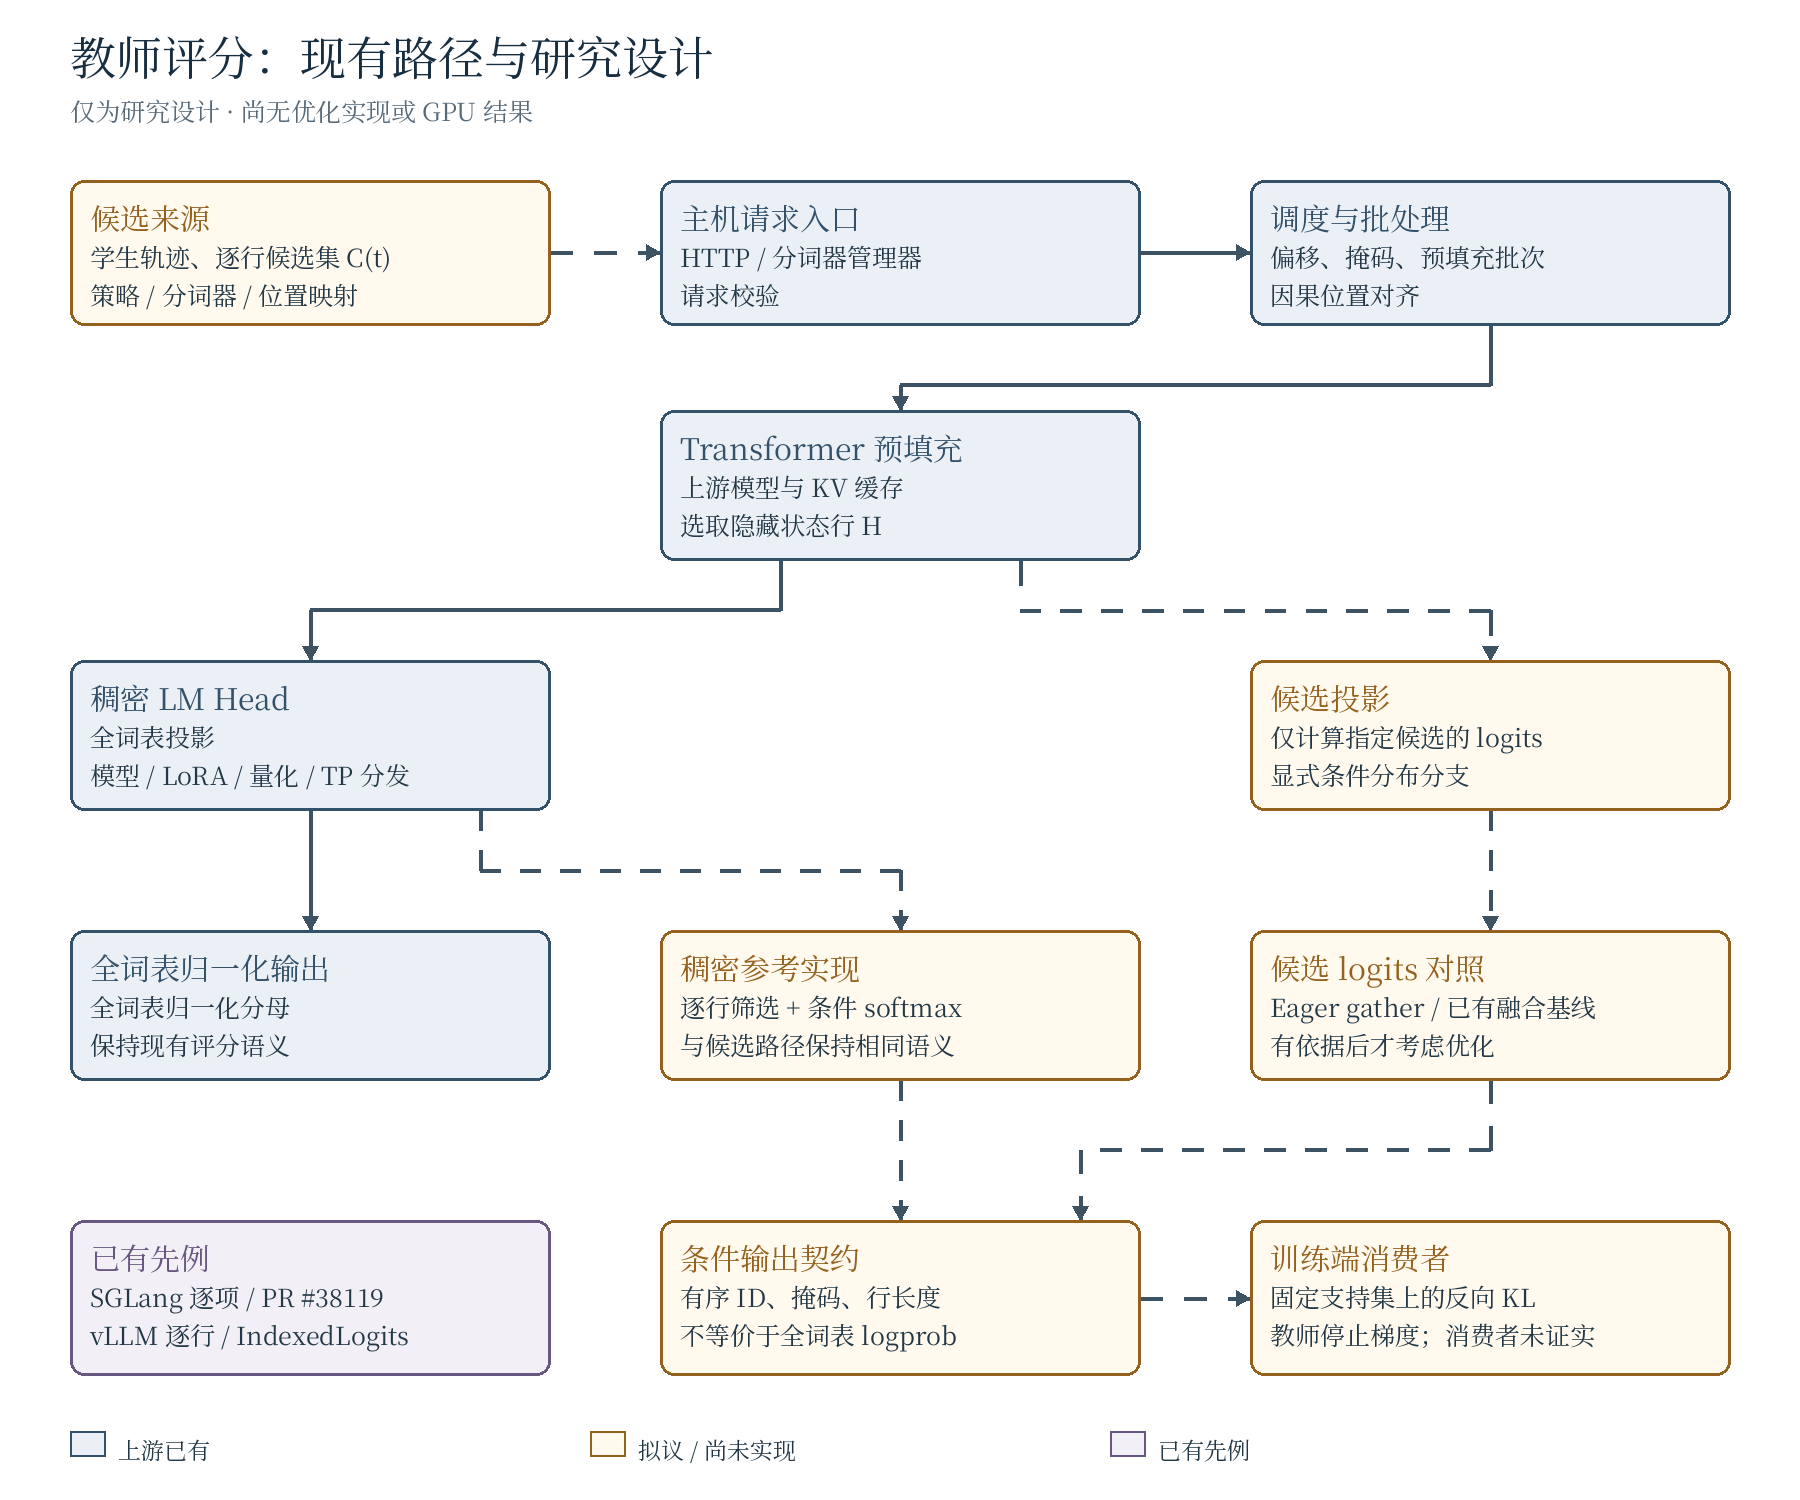
\includegraphics[width=0.92\linewidth,height=0.69\textheight,keepaspectratio]{docs/architecture/architecture.zh-CN.png}
\caption{使用同一拓扑生成的中文标签图。虚线拟议路径尚未实现。}\label{fig:arch}
\end{figure}
\section{解析成本模型}
当每行候选数均为 $K$，忽略 bias 和其他变换时，近似运算量为 $2RVd$ 与 $2RKd$。实际时间取决于有效算力、内存流量、启动、校验和打包。如果可优化部分占基准请求时间的比例为 $f$，其加速倍数为 $s$，则末式为 Amdahl 定律：
\CostEquations
FLOP 比例不能直接预测延迟：稠密矩阵乘法可高效复用权重，而不规则 gather 可能浪费带宽并增加启动次数。完整模型权重通常仍需驻留。候选重叠、批量和形状都可能改变最佳实现。

\textbf{仅为解析示例。} 当 $R=128$、$d=1024$、$V=131072$、$K=32$，每元素两字节时，输出头权重占 256 MiB、稠密 logits 占 32 MiB、eager gathered-weight 张量占 8 MiB、候选 logits 占 8 KiB。这些只是张量大小恒等式，不是实测 GPU 峰值显存。假设 $f=0.1$，即使完全消除该部分，整体请求加速上限也只有 $1/0.9$；实际 $f$ 未知。
\section{评估设计}
在已审核快照中，以下实验均为拟议方案，\textbf{尚未执行}。原生全归一化路径只作为背景；针对相同条件契约比较稠密投影加 gather、分块稠密、eager 索引 gather，以及兼容时的已有 IndexedLogits 实现。未来候选方案应在相关工作负载上胜过正确的强基线，而不是只胜过最慢基线。

先用 CPU FP64 参考检查 logits、归一化、损失和学生梯度。覆盖 $K=1$、$K=V$、候选排列、非法或重复 ID、变长行、掩码、未选 logits 变化和因果偏移一位的情况。在比较实现前确定容差与量化输入；教师值必须停止梯度。不支持的 LoRA、量化或张量并行模式须明确拒绝，或采用保持语义且纳入测量的回退路径。

性能测量需冻结硬件、驱动、框架、模型与分词器版本、轨迹、数据类型、掩码、批处理和计时边界。覆盖候选重叠高低、代表性行数与 prompt 长度、可行并发以及 OOM/回退情况。先建立稳定 A/A 对照，再随机化成对 A/B；保留失败和负结果。分别测量内核及完整 HTTP 请求延迟，包括 p50/p95、吞吐、显存、负载字节数和错误率。分析器应与主要计时分开。仅教师轨迹回放不等于完整训练运行。
\section{限制与判断标准}
已审核快照中，实际消费者以及相对于上述 API 和内核是否仍有缺口均未解决。本项目尚未执行 CPU 数值、梯度、GPU、HTTP 或真实训练实验。当时没有项目加速、显存节省、训练质量收益或原创候选 logits 原语的证据。只有具体消费者、固定语义和相对已有路径的可复现比较共同成立时，剩余缺口才可信；条件不满足时应记录无结论或负结果。

作者已审核仓库版本 \code{c1ab1f4308c2ac1aecf47e222f210a16d0a5a898} 的两份报告；AI 辅助了初稿撰写。后续实质性技术修订须由作者重新审核。源码调查限于所引用快照，并非穷尽式新颖性检索。上游源码和论文归原作者；此处未打包第三方实现。核查范围内 IndexedLogits 仓库未声明许可证，后续复用须另行分析授权。
\section{文档复现}
在仓库根目录安装 XeLaTeX、BibTeX、Poppler、Python 和 Pillow，并按 README 使用随附字体子集后，运行 \code{bash scripts/build_assets.sh} 和 \code{python3 scripts/verify_assets.py}。这些命令只重建文档资产，不运行 SGLang，也不测试研究假设。
\bibliographystyle{plainnat}
\bibliography{docs/reports/references}
\end{document}
